%!TEX root = ../sbc-template.tex
\todo[inline]{Resultado das métricas após o teste dos modelos.}

Inicialmente, fez-se uso da função de ativação \emph{ReLU} para as camadas de saída dos modelos propostos. Os resultados obtidos estão expostos a seguir:

Analisando tais valores, concluiu-se que as redes estavam sofrendo do chamado \emph{ReLU dying problem}, ou problema da morte da \emph{ReLU}. Considerando o gráfico desta função de ativação exibido na Tabela \ref{tab:ativacoes}, nota-se que a \emph{ReLU} exibe saída $0$ para entradas com valores negativos, e saída linear para entradas positivas.
%Sua derivada, também exibida na Tabela \ref{tab:ativações}, é igual a zero para valores negativos e 1 para valores positivos, o que impede os gradientes dos parâmetros da rede calculados na fase \emph{backwards} do treinamento, exibida no Algoritmo \ref{alg:backpropagation}, de tenderem a zero, o que causaria a estagnação da atualização dos parâmetros e consequentemente do aprendizado do modelo.
Apesar dos benefícios da utilização desta função de ativação, os valores de entrada negativos geram saídas e gradientes nulos, o que significa que os parâmetros correspondentes a tais entradas não serão ativados nem atualizados. Isto pode levar a valores nulos na camada de saída. As maneiras de contornar este problema incluem utilizar variantes da \emph{ReLU} que não exibam saídas nulas, diferentes estratégias de inicialização e regularização de pesos e \emph{batches}, entre outras. Assim, substituiu-se apenas na camada de saída a \emph{ReLU} por uma de suas variantes, chamada \emph{Leaky ReLU}. Esta função de ativação produz saídas negativas frente a estímulos negativos, como é possível observar na Figura \ref{fig:lrelu}.

\begin{figure}[h!]
     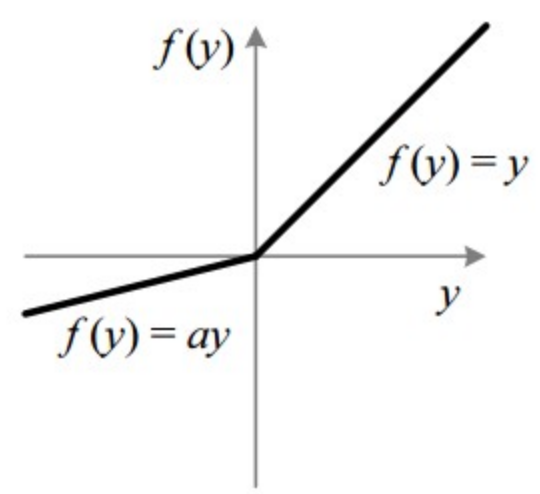
\includegraphics[widht=0.5]{img/lrelu}
     \caption{Função de Ativação \emph{Leaky ReLU}}
     \label{fig:lrelu}
\end{figure}

Os RMSEs obtidos na fase de testes para estas redes podem ser observados na Tabela \ref{tab:results_leaky}

\begin{table}
     \caption{Resultados preliminares do treino e teste dos modelos propostos utilizando \emph{Leaky ReLU} na camada de saída.}
     \label{tab:results_leaky}
     \begin{tabular}{l l}
          Modelo & RMSE \\
          LeNet & $41.55$ \\
          AlexNet & $14.38$
     \end{tabular}
\end{table}
